\section{Architecture}

In this chapter we will present the technical aspects of the game: how the
server and the client are structured, what makes them tick and how they
communicate. We will first analyze the inner workings of the server, then those
of the client and thereafter present the communication in between.\newline

\subsection{Server}


The server exists for relaying the information in between clients. It does not
store state, nor does it validate anything - with one exception: it verifies the
game start condition and only sends the signal to start the game when it
is.\newline

Its main role is to manage connections and resend messages - this means
receiving updates from a single client and then unicasting, multicasting or
broadcasting them. All this is done via TCP.\newline

\subsubsection{Managing connections}

For each incoming connection, the server first checks if the game is in
progress (because it is a prototype, the server only hosts one game). If it is,
the new connection is rejected. Otherwise, it is accepted. The server holds a
HashMap of InetSocketAddress instances holding the IP addresses and ports of the
remote ends of the connections it manages as keys and the unique UUIDs it has
generated for them as values. If an existing IP:port pair is found, that player
is removed and substituted for the new one. In both cases, the new player is
'created': He receives a new unique UUID and is added to the dictionary of
connections. Then, he receives a MessageReceiver and a MessageSender instance,
both added to separate HashMaps with his InetSocketAddress as key. Then, an
<InetSocketAddress, Date> pair is added to a HashMap that remembers the
heartbeats.\newline

Now that the management of this particular connection is up and running, the
MessageReceiver is listening for incoming messages. The messages themselves will
be discussed in further detail below. For now, we can make a differentiation
between heartbeat messages and all the rest. For the case of the heartbeat
messages, on receipt the Date value is updated in the heartbeats HashMap. The
rest of the messages are processed and, according to their type, are sent to
one, many or all the MessageSenders, thus unicasting and mimicking multicasts
and broadcasts. TCP is connection oriented and thus does not allow multicasts
and broadcasts. This issue has been solved by using the list of MessageSenders
and sending to multiple clients through their individual connections.\newline

The heartbeats are periodically checked by a HeartbeatListener, which is a
separate Thread running a continuous loop of periodic checks (200ms in our
case) over all the connections' heartbeats. If the interval from the last update
to the time of the check is larger than a previously established timeout
interval (in our case, it is a fixed 5000ms), the connection will be closed. By
closing the connection, we mean closing the inputs and outputs of the
communication socket, removing all communication objects and connection
record and ultimately the heartbeat records.\newline

The connection lifecycle is depicted in Figure \ref{fig:connectionLifecycle}.

\begin{figure}
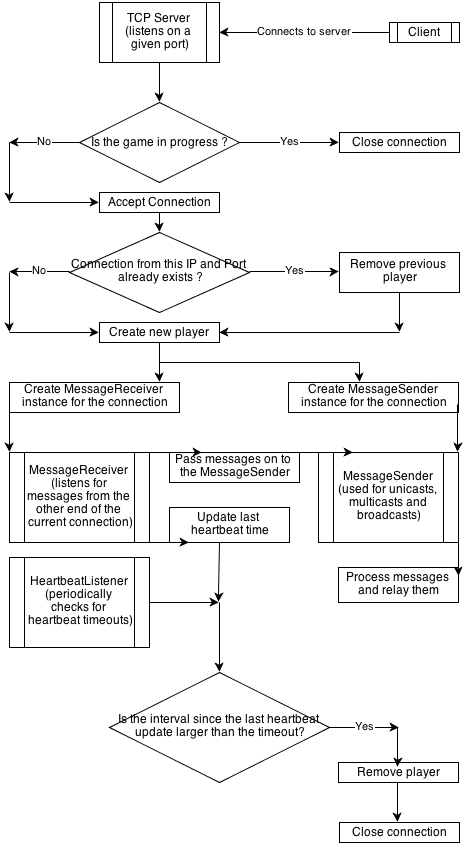
\includegraphics[height=9.00in,width=5.00in]{./images/diagrams/connection_lifecycle.png}  
\caption{\small \sl Connection lifecycle \label{fig:connectionLifecycle}}
\end{figure}

\subsubsection{Relaying messages}

The server serves as a relay, in order to lower the bandwidth and
resource consumption on the mobile clients. The messages exchanged are in
JSON format and have the following base structure: \{messageType: messageNumber,
data: \{\}\}. All clients that are connected to the server send messages
according to the stages they are in. We can discretize three stages: connection,
lobby and game. The server does not make this differentiation - it just relays
what comes, according to the specifics of the messages. To this end, the
MessageReceiver checks which type the message is and if it is the case, extracts
the data into a String and sends it to the MessageSender. The MessageSender will
then reconstruct the message and add further fields to the JSON structure, such
as the UUID of the sender. Then, according to the type of message, it will be
sent as unicast, multicast or broadcast. The unicast is sent via the designated
MessageSender. Multicasts and broadcasts are sent as unicasts through many or
all the MessageSenders available. Multicasts are, for now, useful just for
in-game messages - teams communicate within.\newline

An exception from this flow is made by heartbeat messages. On receipt, the
MessageReceiver takes the date of receipt and updates the entry in the
heartbeats HashMap. The heartbeats HashMap is checked by the HeartbeatListener,
which closes the connection if the last received heartbeat update is older than
a given timeout interval.\newline


\subsection{Client}

The client is the mobile application. It now works with Android versions from
2.3 up. It is structured in six modules, as seen in Figure \ref{fig:clientModules}:

\begin{figure}
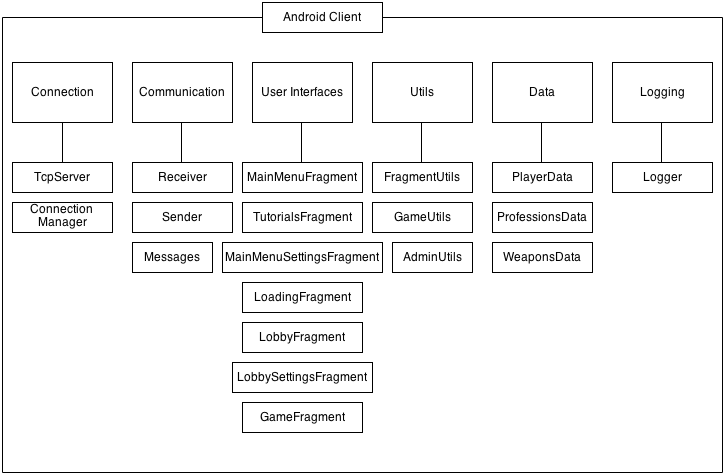
\includegraphics[height=4.08in,width=6.23in]{./images/diagrams/client_modules.png}  
\caption{\small \sl Client modules \label{fig:clientModules}}
\end{figure}

\begin{enumerate}
  \item \textbf{Connection} is responsible with starting and managing the
  connections. Implicitly, it interferes with the Communication module, starting
  and closing the Receiver and Sender objects.
  
  \item \textbf{Communication} is responsible with receiving and interpreting
  messages and sending them. It contains a list of messages that are to be
  treated, organized by context and source (lobby and game, then from and to
  server).
  
  \item \textbf{User Interfaces} are the 'screens' that the player sees in the
  app. They are structured by purpose and interlinked. Some interaction among
  Fragments is done through functions in FragmentUtils.
  
  \item \textbf{Utils} are the helper classes that provide generic methods.
  One class is provided for each purpose: FragmentUtils, GameUtils, AdminUtils.
  
  \item \textbf{Data} is composed of static classes holding information about
  the players in the game, their status, available professions and weapons. Also
  safe access to the data is provided through methods present in these classes.
  
  \item \textbf{Logging} contains just the Logger class, which is responsible
  for logging crashes and data usage.
\end{enumerate}

The client keeps track of state and performs checks and validation such as
in-game shooting, distance checks, enabling powerups, running cooldowns
etc.\newline

The UI of the client app is split into the 7 fragments presented under 'User
Interfaces' in Figure \ref{fig:clientModules}. When the app is run, the first
screen is the main menu. A check will be made if the prerequisits for
playing the game are met(having Google Play Services installed and the
GPS turned on). If either one is not met, a dialog will help the player
quickly get the Google Play Services or turn on the GPS. Buttons in the main
menu provide navigation to the main menu settings, tutorials or lobby(provided
there is an Internet connection). The tutorials provide some insight on what the
game is and how it is played. The settings screen is a temporary solution for
manually giving the IP address and port of the server to which the client is to
connect. The 'Connect to server' button triggers a connection attempt. The
LoadingFragment will be briefly presented, while the connection is established
and some communication is done in the background. Once this is done, the
LoadingFragment is replaced by the LobbyFragment. Here, the player can choose
between teams and edit his character details via the LobbySettings screen. Once
this is also done, the player will signal the fact that he is ready via the
'Ready' button available on the screen. If all players are ready, the server
will send a countdown, followed by a message signalling game entry. This is when
the LobbyFragment is replaced by the GameFragment. The whole game UI is
available at this time, with the exception of the weapon buttons. At this point,
the server will make a check on whether the teams are far enough from each
other. When the teams get far enough from each other, the server will send the
signal to start the game. This is when the game buttons are enabled and the
skirmish begins. The two teams will attempt to eliminate each other through the
use of 'weapons', 'powerups' and strategy.\newline

The UI and technical aspects of the client will be discussed below.\newline


\subsection{Communication}

Communication in between client and server is done via TCP connections that are
kept alive all along the game. The server manages a separate connection with
every client. The messages are in the JSON format and are serialized and
deserialized with the Jackson library.\newline

For each connection, the server creates a Sender and a Receiver objects, each
acting autonomously - their lifecycle is managed by the server. The Receiver
receives more responsibility, as it can close the entire connection or call the
Sender(or a subset of the full number of Senders, in the case of a broadcast or
multicast) to deliver messages.\newline

In addition to the Sender and Receiver objects, a 'heartbeat monitor' object is
running in the background and checking the liveness of all the connections. A
client sends periodic heartbeat messages to show that it is still alive. The
'heartbeat monitor' is responsible for closing the connections that have not
sent a heartbeat update in a given time frame - 3,5 or 10 second frames have
been tried out.\newline

All messages have the following JSON structure: \{messageType: messageNumber,
data: \{\}\}. We are now interested in the data structure. The messageType is a
number that both client and server recognize(as the Messages class is
common).\newline

The Server is active in the message exchange only for the basic administration
purposes: Once a player connects, he receives a configuration json containing
the available 'weapons', 'professions' (with all their attributes) and the list
of already-connected players. It also broadcasts a message telling the existing
players that a new one has connected. When a player disconnects or is
disconnected from the server, a message telling the others that he is
disconnected is sent automatically by the server. Otherwise, the server acts as
a relay.\newline

The Messages class contains a number of inner classes, for proper
classification. We will present the structure, the message types and their
specific JSON structures within:

\begin{enumerate}
  \item \textbf{InGame.ToServer}  
  \begin{enumerate}
    \item CHANGE\_POSITION :
    \{latitude: newLatitude, longitude: newLongitude\}
    
    \item SHOOT :
    \{target: targetUUID, weapon: weaponName, (optional)timestamp: timeStamp\}
        
    \item MESSAGE\_TEAM :
    \{message : messageString\}
      
  \end{enumerate}  
  
  \item \textbf{InGame.FromServer}  
  \begin{enumerate}
    \item CHANGE\_POSITION :
    \{player: playerUUID, latitude: newLatitude, longitude: newLongitude\}
    
    \item SHOOT :
    \{player: playerUUID, target: targetUUID, weapon: weaponName, damage:    
    damageAmount, (optional)timestamp: timeStamp\}
    
    \item MESSAGE\_TEAM :
    \{player: playerUUID, message: newMessage\}
    
    \item GAME\_START :
    \{\} 
        
  \end{enumerate}  
  
  \item \textbf{Lobby.ToServer}
  
  \begin{enumerate}
    
    \item MESSAGE\_ALL :
    \{message: messageString\}
    
	\item CHANGE\_NAME :
	\{name: newName\}
			
	\item CHANGE\_TEAM :
	\{\}		
	
	\item CHANGE\_PROFESSION :
	\{profession: newProfession\}
	
	\item CHOOSE\_WEAPONS :
	this will be made available in further versions where there will be more
	weapons from which to choose
	
	\item READY :
	\{ready : true/false\}    
     
  \end{enumerate}
  
  
  \item \textbf{Lobby.FromServer}
  
  \begin{enumerate}
    	\item ENTER\_GAME :
    	\{\}
		
		\item MESSAGE\_ALL :
		\{player: playerUUID, message: messageString\}
		
		\item CHANGE\_NAME :
		\{player: playerUUID, nickname: newName\}
		
		\item CHANGE\_TEAM :
		\{player: playerUUID, team: newTeam\}
				
		\item CHANGE\_PROFESSION :
		\{player: playerUUID, profession: newProfession\}
		
		\item READY :
		\{player: playerUUID\}
										
		\item PLAYER\_JOINED :
		\{player: playerUUID, name: playerName\}
		
		\item PLAYER\_LEFT :
		\{player: playerUUID\}
			
		\item CONFIGURATION :
		A huge JSON thing that the Server composes based on a Config file and sends it
		to the client. 
		
		\item COUNTDOWN :
		\{secondsLeft: numberOfSecondsLeft\}
		
  \end{enumerate}  
  
\end{enumerate}

The communication and action flow on the server, newly joined client and
existing clients is presented in Figure\ref{fig:client_server_flow}

\begin{figure}
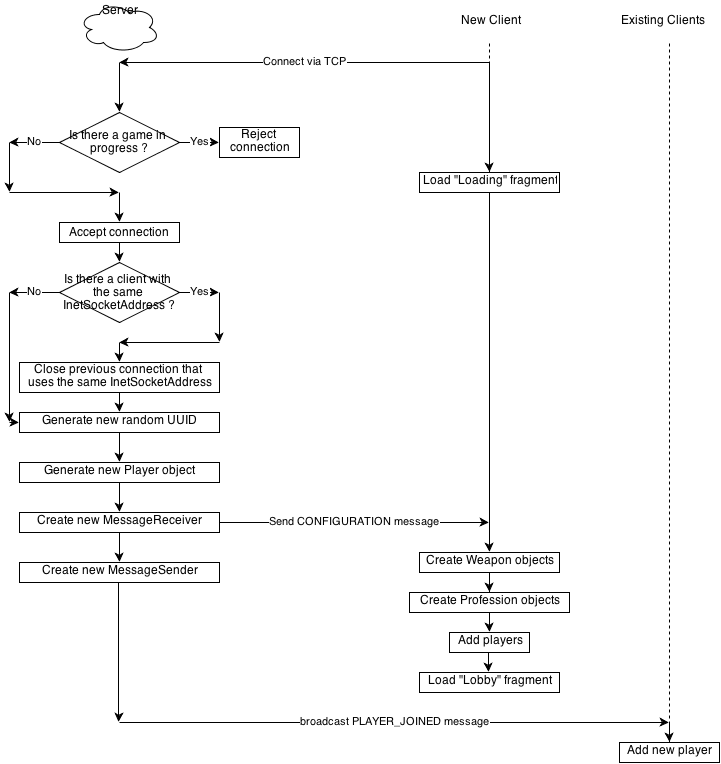
\includegraphics[height=7.665in,width=6.23in]{./images/diagrams/Client-Server.png}
\caption{\small \sl A new client joining the game
\label{fig:client_server_flow}}
\end{figure}
